% Document class, language and encoding setup
\documentclass[a4paper,12pt,danish]{report}

\usepackage[danish]{babel}
\usepackage[utf8]{inputenc}
\usepackage[T1]{fontenc}
% Fixing the font issue
\usepackage{ae,aecompl}

% Color package
\PassOptionsToPackage{dvipsnames}{xcolor}
	\RequirePackage{xcolor} % [dvipsnames] 
	
% Allows page-links in pdf file
\usepackage[colorlinks=true]{hyperref}

\usepackage{pdfpages}
% Todo notes package and commands
\usepackage{todonotes}
% Allows commands to emit a space "at the end"
\usepackage{xspace}

% Listings setup
\usepackage{listings}

% Graphics setup
\usepackage{graphicx}
\graphicspath{{./graphics/}{./graphics/sensor/}}

\usepackage{tikz}
\usetikzlibrary{calc}
\usepackage{amsmath}
\usepackage{amssymb}

% Advanced tables
\usepackage{tabularx}

% Clever references
\usepackage{cleveref}

% Bibliography
\usepackage[square,numbers]{natbib}
\bibliographystyle{plainnat}

% Force position [H]
\usepackage{float}

% For figures with sub-figures
\usepackage{subcaption}

% Tikz
\usepackage{tikz}
\usetikzlibrary{arrows,backgrounds,snakes}
 
% Additional commands
\input{./setup/todonotes}
% Her er en liste over navnene p� de forskellige styles
% C#: csharp
% F#: fsharp

% 
% Listings kan refereres vha. \cref{}
\crefname{listing}{kodeeksempel}{kodeeksempler}
\Crefname{listing}{Kodeeksempel}{kodeeksempler}
% 

%Algoritmer i cref
\crefname{algocf}{algoritme}{algoritmer}
\Crefname{algocf}{Algoritme}{Algoritmer}
%

\lstdefinestyle{standard}
{
	frame=shadowbox,
	framesep=5pt,
	rulecolor=\color{blue!40!black},
	rulesepcolor=\color{white!93!black},
	basicstyle=\ttfamily\normalsize,
	numbers=left,
	numberstyle=\tiny,
	numberfirstline=true,
	%numberblanklines=false,
	stepnumber=1,
	numbersep=9pt,	
	captionpos=b,
	escapeinside={(*}{*)}
}

\lstdefinestyle{c}
{
	style=standard
}

\lstdefinestyle{csharp}
{
	style=standard,
	language=[Sharp]C
}
\lstdefinestyle{csharpsmall}
{
	style=csharp,
	basicstyle=\ttfamily\footnotesize
}
\lstdefinestyle{fsharp}
{
	language=[Sharp]F,
	frame=lr,
	rulecolor=\color{blue!80!black}
}
\lstdefinestyle{fsharpsmall}
{
	style=fsharp,
	basicstyle=\ttfamily\footnotesize
}
%Definitions
\newcommand{\mindsqualls}{MindSqualls\xspace}
\newcommand{\csharp}{\textsc{C\#}\xspace}

\newcommand{\lstref}[1]{liste \ref{#1}}

%Superscript and subscript
\newcommand{\superscript}[1]{\ensuremath{^{\textrm{#1}}}}
\newcommand{\subscript}[1]{\ensuremath{_{\textrm{#1}}}}

\begin{document}
\listoftodos[Todo liste]
\pagenumbering{roman}
%Front page
\begin{titlepage}
\newcommand{\HRule}{\rule{\linewidth}{0.5mm}}

\begin{center}

\HRule \\[0.5cm]
\textsc{ \Huge Mapping}\\

\HRule \\[1cm]

\textsc{\Large SW505E13}

\vfill
{\Large Udvilking af komplekse softwaresystemer}
\\ ~\\
{\large Efterårssemesteret 2013}

\end{center}
\end{titlepage}

\clearpage

\thispagestyle{empty}
\begin{titlepage}
\setlength{\textwidth}{15cm}
	\noindent
\begin{nopagebreak}
{\samepage 
\begin{tabular}{r}
	\parbox{15cm}{\raisebox{11mm}{\includegraphics[height=1.2cm]{./graphics/aauLogoDa.jpg}}
	\hfill \parbox{7cm}{\begin{tabular}{l}
		{\small \textbf{Institut for Datalogi}}\\
		{\small Selma Lagerløfs Vej 300} \\
		{\small 9220 Aalborg Ø} \\
		{\small Phone (+45) 9940 9940} \\
		{\small Fax (+45) 9940 9798} \\
		{\small http://cs.aau.dk}
	\end{tabular}}
.	}
\end{tabular}

\begin{tabular}{cc}
	\parbox{8cm}{
	\begin{description}
		\item { \textbf{Titel:}}\\ 
			Mapping
			\mikael{Bør vi ikke finde en bedre titel?}
    		\item { \textbf{Tema:}}\\ 
			\raggedright Indlejrede systemer
	\end{description}
	
	\parbox{8cm}{
	\begin{description}
		\item { \textbf{Projektperiode:}}\\
			01-09-2013 -\\
			20-12-2013
 		\hspace{4cm}
		\item { \textbf{Projektgruppe:}}\\
  			sw505f13
 		\hspace{4cm}
		\item {\textbf{Deltagere:}}\\
			Anders R. Nielsen\\
			Bruno Thalmann\\
			Mikael E. Christensen\\
			Mikkel S. Larsen\\
			Stefan M. G. Micheelsen\\
			Stefan M. Thilemann\\
		\hspace{2cm}
		\item { \textbf{Vejleder:}}\\
 			Nicolaj Søndberg-Jeppesen\\
  	\end{description}
	}
	\begin{description}
		\item { \textbf{Printings:} 2}
		\item { \textbf{Pages:} \pageref{LastPageBody} } 
		\item { \textbf{Appendices:} 40}
		\item { \textbf{Total pages:} \pageref{LastPage} }
		\item { \textbf{Source code:} \url{https://github.com/deaddog/sw505-code/tree/v1.0}}
		\bruno{husk at opdatere dette.}
	\end{description}
	\vfill } &
	\parbox{6.5cm}{
 	 \vspace{.15cm}
  	\hfill 
  	\begin{tabular}{l}
  		{Abstract:}\bigskip \\
  		\fbox{
  		\parbox{6cm}{\bigskip
     		{\vfill{\small \paragraph{Purpose:}The purpose of this project was to map an unknown area using a robot, which location is given by an external device and thus, always known.

\paragraph{Method:}To accomplish this, a robot was built using \legoms, consisting of a rotating ultrasonic sensor construction built on top of robot.
The purpose of the robot was to navigate and collect sensor measurements and provide these to a PC, which would construct a map based on the supplied data.
This would result in a continuously updated occupancy grid, by using a simple- or Gaussian sensor model).
Additionally, as a simplification of the problem, a PC would supply the robot with its location and orientation (pose), based on color-tracking a live stream from a Kinect, whenever needed.\thilemann{sidste del bør omformuleres}

\paragraph{Results and conclusion:}
\mikael{Noget test-resultat og konklusion}
     		\bigskip}}
     	}}
   	\end{tabular}}
\end{tabular}
\noindent{\footnotesize{\textit{Rapportens indhold er frit tilgængeligt, men offentliggørelse (med kildeangivelse) må kun ske efter aftale med forfatterne.}}}
}%samepage end
\end{nopagebreak}
\end{titlepage}

\clearpage

\newcommand{\prefaceHeaderName}{Forord}
\section*{\prefaceHeaderName}
\addcontentsline{toc}{subsection}{\prefaceHeaderName}
Her skal der være et forord
\bruno{husk at skrive dette.}

\clearpage


%Table of content
\tableofcontents

\clearpage

\pagenumbering{arabic}

\newcommand{\introductionHeaderName}{Introduktion}
\section*{\introductionHeaderName}
\addcontentsline{toc}{subsection}{\introductionHeaderName}
Her skal der være en introduktion.

\clearpage

\part{Analyse}
%Sets first chapter to one instead of zero

\chapter{Platform}
I dette kapitel vil den valgte platform, \legoms, blive kort beskrevet med en begrundelse for dette valg.
Yderligere vil der blive argumenteret for valg af API til NXT-enheden.

\section{Lego Mindstorms}\label{lego:mindstorms-nxt}
\legoms er et byggesæt, hvor det er muligt at bygge programmerbare robotter i \lego-klodser.

Til at bygge disse robotter er der i \legoms nogle sensorer og aktuatorer. Sensorerne gør det muligt for robotten at modtage input fra sine omgivelser.
Ved brug af aktuatorerne kan robotten reagere på disse inputs.

Ud over de originale \lego dele er der også tredjeparts forhandlere, som har et udbud af andre sensorer og aktuatorer. \thilemann{Enten bør denne linje fjernes, eller også skal vi skrive om sådanne sensorer?}

\subsection{NXT}
Denne sektion er baseret på \cite{nxt}, hvilket omhandler NXT 2.0, som er den version der bruges i dette projekt.
NXT Intelligent Brick (oftest kaldt blot 'NXT' eller 'brick') er hjernen i \legoms robotten.
Det er den der står for at modtage og behandle input fra sensorer samt styre de monterede aktuatorer.
Et billede af NXT 2.0 kan ses i \cref{platform:nxt}.

\begin{figure}
\begin{center}
\includegraphics[scale=.5]{./graphics/nxt/brick}
\end{center}
\caption{'NXT Intelligent Brick'}
\label{platform:nxt}
\end{figure}

\subsubsection{Porte}
NXT'en har 3 motor porte (kaldet A, B og C) og 4 sensor porte (kaldet 1, 2, 3 og 4).

\subsubsection{Tilslutningsmuligheder}
Der kan kommunikeres med NXT'en ved at tilslutte den til en anden enhed med USB-kabel eller Bluetooth\textregistered.

\subsubsection{Feedback}
Til output har NXT'en en 100 x 64 pixel LCD display samt en 8 kHz højttaler.

\subsubsection{Styring}
NXT'en kan styres på to måder:
Man kan sende kommandoer og modtage beskeder (for eksempel sensor aflæsninger) på en ekstern enhed (oftest en computer eller en anden NXT).
Alternativt kan programmer sendes (via Bluetooth eller USB) til NXT'en, hvorfra de kan køres direkte, uafhængig af eksterne enheder.


\subsubsection{Tekniske specifikationer}
De tekniske specifikationer for NXT 2.0 kan ses på \cref{mindstorms:tekniske_spec} \cite{nxt}. 


\begin{figure}
\begin{tabular}{|c |c|}
\hline
Microcontroller & \shortstack{\\32-bit ARM7 microcontroller\\ 8-bit AVR controller}\\
\hline
RAM & \shortstack{ \\256 Kb FLASH, 64 Kb RAM \\ 4 Kb FLASH, 512 b RAM} \\
\hline
Kommuniation & \shortstack{ \\Bluetooth (Bluetooth Class II V2.0 compliant) \\ USB full speed port (12 Mbit/s)}\\
\hline
Input porte & 4 \\
\hline
Output porte & 3 \\
\hline
Display & 100 x 64 pixel LCD \\
\hline
Højttaler & 8 kHz lyd. 8-bit lydkanal og 2-16 kHz sample rate\\
\hline
Strømkilde & 6 AA batteries\\
\hline
\end{tabular}
\caption{LEGO MINDSTORMS NXT tekniske specifikationer}
\label{mindstorms:tekniske_spec}
\end{figure}


\subsection{Valg af \legoms}
Der er mange gode grunde til at vælge \legoms.
Her er givet fire overordnede punkter, der vil blive gennemgået efterfølgende:

\begin{itemize}
\item{Tilgængelighed}
\item{Nemt at gå til}
\item{Stort udvalg af sensorer}
\item{Mange muligheder ift. styring}
\end{itemize}

\subsubsection{Tilgængelighed}
Grundet at \lego (inkl. \legoms) er ment til almindelige brugere, er det masseproduceret og kan derved købes forholdsvist billigt og i helt almindelige butikker (legetøjsforretninger og ofte også supermarkeder).

\subsubsection{Nemt at gå til}
Det faktum at man bygger sin robot i \lego klodser, med tilføjelse af \legoms sensorer/aktautorer gør det nemt at lave en konstruktion og derefter modificere den så den udfører sin opgave tilfredsstillende.

Denne høje versatilitet gør at \lego er perfekt til en prototype-orienteret fremgangsmåde for bygning af robotter.

\subsubsection{Stort udvalg af sensorer}
På grund af det store udvalg af sensorer kan man bygge robotter der kan løse et væld af opgaver.
Ved et projekt med høj usikkerhed, er det derved også nemt og billigt at udskifte en sensor.

\subsubsection{Mange muligheder ift. styring}
Her menes der både overordnet den måde hvorpå robotten styres, men især også den måde hvorpå NXT'en styres.
NXT'en kan udstyres med brugerdefineret firmware, der giver utroligt mange muligheder (og dermed også fleksibilitet) ift. hvordan den kan styres.

I afsnittet herefter vil der blive argumenteret for valg af API, hvor API her skal forstås som måden hvorpå robotten skal styres.

\section{Valg af NXT API}\label{nxt_api}
Den ideelle løsning ville være at vælge et system, hvor robotten styrer alt; både navigation og indsamling af sensor-målinger og selve kortlægningsdelen.
Dog er der begrænset med plads til data på NXT'en (256 KB flash, 64 KB RAM), samtidig med at dens regnekraft heller ikke er så god (32-bit ARM7 microcontroller).\thilemann{Måske skulle der nævnes hvor langsom den er?}
På grund af robottens hardwaremæssige begrænsninger og at problemformuleringen siger at robotten til enhver tid skal kende sin position, er det derfor nødvendigt at 'outsource' visse opgaver til en PC.
Dette ses blandt andet ved at der benyttes en Microsoft Kinect til at lokalisere robotten, hvilket gør en PC påkrævet for at bearbejde billeddata fra Kinecten for netop at fortælle robotten dens faktiske position.

Grundet disse begrænsninger og givet problemet der skal løses, ville der sagtens kunne laves et to-delt system.
Den ene del bestående af selve robotten, som skal navigere sig rundt i verden og bruge sine sensorer til at opfatte verden omkring sig.
Den anden del, som består af selve kortlægningen, kræver mere plads til data, samt større beregningskraft.

\subsubsection*{Overordnet valg}
For at kunne overholde ovenstående, skal der kunne laves et to-delt stykke software, hvor den ene del kører på robotten og den anden del på en stærkere platform, i vores tilfælde en PC.

Det der så skal vælges nu, er hvordan det software der skal køre på robotten skal laves, samt det software der skal køres på PC'en.
Vigtigt er at det skal være muligt for den ene del at kommunikere med den anden, da der skal kunne sendes kommandoer til robotten fra PC'en, samt at PC'en skal kunne modtage sensor-input fra robotten.

\subsubsection*{NXC}
Til det software der skal køres på robotten har vi valgt NXC, da det er simpelt og dækker alle behov.
NXC-programmer skrives i et C-lignende sprog, hvorefter disse programmer kan sendes til NXT'en og køres direkte der på.
Der er også stor mulighed for kommunikation mellem NXC-programmer og eksterne programmer.
Dette gør det muligt at skrive et program til NXC'en, hvorefter der kan udføres forskellige handlinger afhængig af hvad PC'en beder den om.
Der vil blive gået mere i dybden med NXC i \cref{nxc}.

\subsubsection*{MindSqualls}
Til det software der skal køres på PC, altså det der skal sørge for selve opdateringen og beregningen af kort, har vi valgt \mindsqualls.
\mindsqualls er et .NET bibliotek skrevet i \csharp, hvori det er muligt at kommunikere med en NXT, både ved at sende direkte kommandoer eller via abstraktion over NXTens aktuatorer/sensorer opfattet som objekter.
Valget faldt på \mindsqualls da dette var simpelt og dækkede alle behov ift. kommunikation med NXT.
Desuden har gruppen stor erfaring med \csharp og Visual Studio, hvilket også ses som værende en stor fordel.
\mindsqualls vil blive uddybet i \cref{mindsqualls}.

\chapter{Sensorer}
% !TeX spellcheck = da_DK
\label{sensorer}
Følgende afsnit undersøger de tilgængelige sensorer og motorer, som er interessante for projektet.
Da der er stor forskel på sensorerne, der er til rådighed, er der foretaget forskellige forsøg, hvis formål er at klarlægge præcisionen af de forskellige sensorer.

\begin{figure}[h]
\centering
\begin{subfigure}[b]{.4\textwidth}
\centering
\includegraphics[width=.5\textwidth]{us}
\caption{Ultrasonisk sensor}
\label{sensor:ultrasonic_sensor}
\end{subfigure}
\begin{subfigure}[b]{.4\textwidth}
\centering
\includegraphics[width=.5\textwidth]{infrared_sensor}
\caption{Infrarød sensor}
\label{sensor:infraroed_sensor}
\end{subfigure}
\begin{subfigure}[b]{.4\textwidth}
\centering
\includegraphics[width=.5\textwidth]{lego_motor}
\caption{Servomotor}
\label{sensor:servo_motor}
\end{subfigure}
\begin{subfigure}[b]{.4\textwidth}
\centering
\includegraphics[width=.5\textwidth]{hitechnic_compass}
\caption{Kompas}
\label{sensor:compass}
\end{subfigure}
\caption{Komponenter der betragtes til konstruktion af robotten.}
\end{figure}

\section{Afstandssensorer}
\mikael{I kompas konkluderer vi at det ikke kunne bruges. Vi konkluderer ikke noget for hverken afstandssensor eller motor, bør vi ikke det?}
\bruno{uenig - konklusion for aftstandssensorer er at finde under sammenligning af afstandssensorer. Med motor er der ikke så mange alternativer så de rbeskriver vi bare usikkerheden.}
Dette afsnit beskriver testen af de to afstandssensorer (\cref{sensor:ultrasonic_sensor,sensor:infraroed_sensor}), som kan være interessante at montere på robotten.
For at afgøre hvilken der passer bedst til at løse problemet, er de blevet testet.

Formålet med at teste disse sensorer er, at robotten skal have en måde at afgøre på, hvor langt der er til objekter omkring den.
Derfor vil disse tests undersøge følgende:
\begin{itemize}
\item Hvor nøjagtigt kan sensorerne bestemme afstanden til et objekt?
\item Hvilket interval kan der måles i (hvad er den minimale og maksimale måleafstand)?
\end{itemize}

\subsection{Ultrasonisk Sensor}
Den ultrasoniske sensor, som kan ses på \cref{sensor:ultrasonic_sensor}, kan måle afstand til objekter.

Det gøres ved at sende en lydbølge, hvorefter der beregnes hvor lang tid det tager for denne at ramme objektet, for derefter at blive reflekteret tilbage igen.
Den maksimale afstand der kan måles er 255 cm, med en præcision på $\pm 3$ centimeter.
De bedste aflæsninger fåes ved måling af store flade objekter med hård overflade, i modsætning til mindre objekter med rund og/eller blød overflade.\cite{nxt}

\subsubsection{Test}
Der er gennemført en mindre test af sensoren, for at finde ud af hvor nøjagtig den er.

Testen blev udført ved at lave en simpel \lego konstruktion, kun bestående af NXT og den ultrasoniske sensor.
Konstruktionen blev placeret i en bestemt afstand fra en væg, hvor sensoreren var placeret vandret, pegende direkte på væggen.
Herefter blev sensoren aflæst, samtidig med at afstanden mellem væg og sensor blev målt med lineal.
Der blev udført den samme test 3 gange, hver gang for en bestemt række afstande mellem 0 og 255 cm.

\subsubsection{Resultater}\label{sensorer:us:resultater} Tabel med resultater fra forsøget kan ses i \cref{appendix:ultrasonisk}.

En graf-repræsentation af resultaterne kan ses i \cref{sensor:ultrasonic_resultat_diagram}.
Den røde linje indikerer det ideele resultat. mens den brune, grønne og lilla linje viser resultaterne fra de tre test.
Det ses på grafen, at de tre test alle giver forkerte resultater, når sensoren er mindre en 20 cm fra objektet.
Desuden kan det ses, at der i test 1 (brun) kun kunne måles op til 170 cm, før der opstod usikkerhed, hvor de andre tests nåede 200 cm (test 2 -- grøn) og 230 cm (test 3 -- lilla) før der opstod større usikkerhed.
Generelt overholder sensoren dens specifikationer, idet der er en afvigelse på 3 cm på målingerne, men forsøget viser, at der kun kan måles mellem 20 og 170 cm, uden der opstår større usikkerheder.

\begin{figure}[h]
\centering
\includegraphics[clip=true, trim = 0cm 2.5cm 0cm 2.5cm,width=\textwidth]{ultrasonicchart}
\caption{Graf over forsøgsresultaterne fra testen af den ultrasoniske sensor.}
\label{sensor:ultrasonic_resultat_diagram}
\end{figure}



\subsection{Infrarød Sensor}
Den infrarøde afstandssensor fra mindsensors.com, som kan ses på \cref{sensor:infraroed_sensor}, er en afstandssensor med høj præcision, der kan måle afstande mellem 10 og 80 cm.
Sensoren virker som den ultrasoniske sensor, men sender et infrarødt lys i stedet for en ultrasonisk impuls.

\subsubsection{Test}
For at afprøve sensorens præcision og rækkevidde, er der foretaget en test af sensoren.

Opstillingen brugt til udførelse af testen bestod af tre A4 ark spændt ud på gulvet ind til en væg. 
Papiret havde markeringer for hver 2 cm fra væggen.

Udførelsen af testen gik ud på at placere en NXT med påsat infrarød sensor ved hver indikator, for derefter at aflæse sensorens måling.
På denne måde blev afmålingen fra sensoren ved en given afstand holdt op imod den egentlige afstand til væggen, som afmålt på papiret.

\subsubsection{Resultater}

Resultaterne fra testen er præsenteret i \cref{appendix:infrared}. 
Disse resultater er vist på \cref{sensor:infrared_chart}.
Den røde graf er den reelle afstand, som aflæst på papiret/med lineal, mens de blå firkanter er målepunkter.
Den sorte graf er en lineær regression over måleresultaterne.

Ud fra grafen ses det, at der er stor usikkerhed i starten og slutningen, hvilket næsten stemmer overens med den lovede rækkevidde på 10 til 80 cm.
De bedste resultater findes dog imellem 8cm og 56 cm. 
Mellem 8cm og 56cm er der maximalt 27 mm afvigelse fra det forventede, (forventet 500, målt 527).

\begin{figure}[h]
\includegraphics[clip=true, trim=0cm 8cm 0cm 8cm,width=\textwidth]{Infraredchart}
\caption{Graf over forsøgsresultaterne fra testen af den infrarøde sensor.}
\label{sensor:infrared_chart}
\end{figure}

\subsection{Sammenligning af afstandssensorer}

Der er nu foretaget test af to forskellige afstandssensorer, den ultrasoniske sensor og den infrarøde sensor. 
Den ultrasoniske sensor var præcis med en afvigelse på $\pm$3 cm mellem 20 cm og 170 cm.
Den infrarøde sensor var præcis med afvigelse på $\pm$3 cm, mellem 10 cm og 56 cm.
Den infrarøde sensor angiver sine målinger med højere præcision, men da fejlmarginen er 3 cm, anses den ikke som værende mere præcis end den ultrasoniske sensor.
I forhold til rækkevidden, måler den ultrasoniske længere væk end den infrarøde, mens den infrarøde sensor måler tættere på end den ultrasoniske.
Valget mellem de to sensorer er derfor afhængig af hvilket krav robotten har til rækkevidden.

\section{Motor}\label{sensorer:motorer}
Motoren, der er testet her, er fremstillet af \lego og kan ses i \cref{sensor:servo_motor}.
Den består af en rotationssensor, som måler omdrejningerne ved grader, med en nøjagtighed på \'en grad i følge \lego. 
Desuden gør denne sensor det også muligt at styre hvor meget kraft motoren skal køre med.
Køres der med flere motorer har NXT'en indbygget software, der gør det muligt at synkronisere disse, hvilket er hensigtsmæssig hvis fx. den ene motor skulle være stærkere eller svagere end den anden.\cite{tikNXT}

\subsection{Formål}
Formålet med denne test er at teste motorens nøjagtighed.
Hvis motoren ikke har høj nøjagtighed, skal der tages højde for det, når den monteres på robotten.

\subsection{Test}
For at bestemme motorens nøjagtighed i praksis, blev en test opstillet hvor to moterer roteres med et bestemt antal grader.
Motorernes egentlige rotation aflæses med vinkelmåler og holdes op mod den ønskede rotation, samt den rotation motorerne angiver at de har roteret.
Sidstnævnte fås ved at aflæse motorernes \lstinline[style=csharp]!TachoCount! egenskab.

\subsubsection{Resultat}
Resultaterne fra forsøget kan ses i \cref{appendix:motor_test}. 
Af resultaterne kan vi bestemme de største afvigelser til +7 og -4 grader.
Tacho-værdien har en afvigelse på maksimalt +1 og -4 grad.
Dette stemmer ikke overens med de antagede $\pm$1 grads afvigelse.

+7 og +6 grader målt optræder kun \'en gang.
Ellers er den maksimale målte afvigelse $\pm$4 grader, men selvom vi antager, at det er pga. unøjagtige målinger ved forsøgsudførelsen, er det stadig ikke $\pm$1 grad.

Kigger vi på \cref{sensor:motor_sensor_diagram} kan vi se, at målingerne ligger længst udenfor det optimale (sorte stiplede linje), hvilket er en god indikator for, at det er bedre at benytte tacho-værdien.

\begin{figure}
\includegraphics[width=\textwidth]{motor_diagram}
\caption{Afvigelser i test-resultaterne.}
\label{sensor:motor_sensor_diagram}
\end{figure}

Desuden kan vi se på samme figur, at motor b er meget mere unøjagtig end motor c.
Ideelt ville de to motorer give det samme resultat.

Dvs. den målte værdi har en afvigelse på $\pm$4 grader, mens tacho-værdien har en afvigelse på +1 og -4 grader, og at synkronisering af de to motorer ikke giver den ønskede effekt.

\section{HiTechnic NXT Kompas Sensor}
Kompasset fra HiTechnic er et digitalt kompas, der måler jordens magnetiske felt.
Kompasset kan returnere en værdi, der repræsenterer kompassets nuværende orientering.
Ifølge HiTechnic er værdierne returneret fra kompasset præcise ned til 1 grad.
Kalibrering skulle desuden ikke være nødvendig.
Dog er det nødvendigt, for at minimere forstyrrelser, at kompasset holdes 10-15 cm væk fra forstyrrende elementer, herunder \lego NXT og motorer.\cite{hitechnic_compass}

I \cref{kompas:precision} undersøges hvorvidt målinger fra kompasset kan leve op til disse oplysninger.

\subsection{Formål}
Formålet med denne test er at undersøge kompassets nøjagtighed.
Hvis kompasset har høj nøjagtighed, kan det monteres på robotten og afgøre hvilken retning denne vender.

\subsection{Kompas Sensor i \mindsqualls}
Til at styre denne sensor i \mindsqualls, skal der bruges en af de seperate klasser til HiTechnic sensorerne, som findes i namespacet \lstinline[style=csharp]!NXT.MindSqualls.HiTechnic!.
Til kompas sensoren anvendes klassen \lstinline[style=csharp]!HiTechnicCompassSensor!.

\subsubsection{Aflæsning af værdier}\label{kompas:reading}
Ved aflæsning af egenskaben \lstinline[style=csharp]!Heading! fra sensores klasse, gives et heltal mellem 0 og 359, der angiver kompassets orientering.
Det har været nødvendigt at ændre implementationen af \lstinline[style=csharp]!Heading!, da den oprindelige implementation ikke aflæste kompassets orientering ned til \'en grad.
Sensoren repræsenterer sin orientering på to forskellige måder.
Begge anvender to bytes.
Den ene metode beskriver afstanden vha. et 16-bit heltal.
Den anden (som var anvendt i implementationen af \lstinline[style=csharp]!Heading!) beskriver afstanden ved at lade den ene byte angive vinklen i intervaller af to grader.
Altså kunne de værdier der aflæses fra denne byte være 0-179, hvilket efterfølgende ganges med 2 for at få den egentlige værdi.
Hertil lægges værdien af den anden byte, der kan have værdien 0 eller 1.
I den oprindelige implementation af \lstinline[style=csharp]!Heading!, er der ikke taget højde for denne ekstra værdi.
Dette er inddraget i test 3 i det følgende afsnit.

\subsection{Præcisionstest}\label{kompas:precision}
For at teste kompas sensoren, er målinger taget fra denne og holdt sammen med målinger foretaget med vinkelmåler.
Sammenligningen er sket ved at tage to målinger med kompasset og sammenligne differencen med den værdi målt med vinkelmåler.
I forbindelse med test af sensoren, blev der udført i alt tre tests:
\begin{enumerate}
\item Kompas monteret på robot med hjul
\item Kompas monteret på fast konstruktion
\item Gentagelse af test 2, med \textit{øget præcision}
\end{enumerate}
Den øgede præcision der beskrives her, dækker over en opdatering af \mindsqualls klassen \lstinline[style=csharp]!HiTechnicCompassSensor!, der blev foretaget efter de første to tests.
Resultaterne fra de tre tests kan ses i tabellerne \ref{kompas:test1:table}, \ref{kompas:test2:table} og \ref{kompas:test3:table} på side \pageref{kompas:test1:table}.

Af resultaterne er der lavet et boksplot (\cref{kompas:boksplot}).
Plottet illustrerer den afvigelse, der var fra de værdier, der blev aflæst af kompasset, til de værdier, der blev målt med vinkelmåler.
Prikkerne på plottet repræsenterer den gennemsnitlige afvigelse.

\begin{figure}[h]
\centering
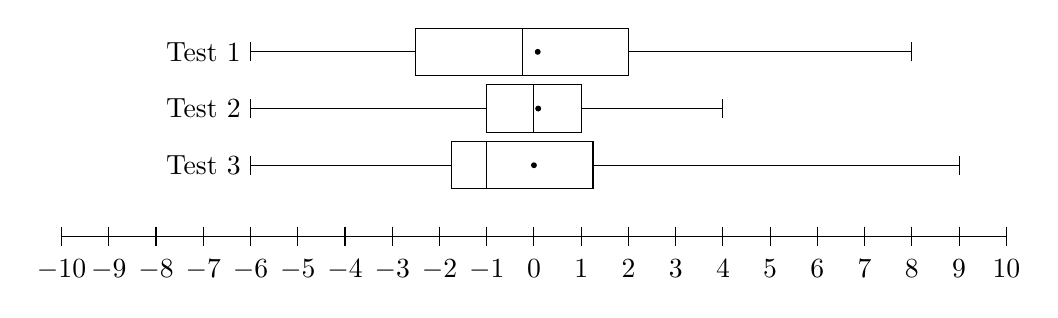
\begin{tikzpicture}[scale=0.6]
%Test 1
\draw (-2.5,3.4) rectangle (2,4.4); % Boks
\draw (-0.25,3.4) -- (-0.25,4.4); % Median streg
\draw (2,3.9) -- (8,3.9); % Fra øvre kvartil til maks
\draw (-2.5,3.9) -- (-6,3.9);% Fra nedre kvartil til min
\draw (8,3.7) -- (8,4.1); % Maksimum vertikal streg
\draw (-6,3.7) -- (-6,4.1); % Minimum vertikal streg
\node[left] at (-6,3.9) {Test 1};
\filldraw[color=black] (0.08,3.9) circle (0.05cm); % Gennemsnittet

%Test 2
\draw (-1,2.2) rectangle (1,3.2); % Boks
\draw (0,2.2) -- (0,3.2); % Median streg
\draw (1,2.7) -- (4,2.7); % Fra øvre kvartil til maks
\draw (-1,2.7) -- (-6,2.7);% Fra nedre kvartil til min
\draw (4,2.5) -- (4,2.9); % Maksimum vertikal streg
\draw (-6,2.5) -- (-6,2.9); % Minimum vertikal streg
\node[left] at (-6,2.7) {Test 2};
\filldraw[color=black] (0.09,2.7) circle (0.05cm); % Gennemsnittet

%Test 3
\draw (-1.75,1) rectangle (1.25,2); % Boks
\draw (-1,1) -- (-1,2); % Median streg
\draw (1.25,1.5) -- (9,1.5); % Fra øvre kvartil til maks
\draw (-1.75,1.5) -- (-6,1.5);% Fra nedre kvartil til min
\draw (9,1.3) -- (9,1.7); % Maksimum vertikal streg
\draw (-6,1.3) -- (-6,1.7); % Minimum vertikal streg
\node[left] at (-6,1.5) {Test 3};
\filldraw[color=black] (0.00,1.5) circle (0.05cm); % Gennemsnittet

% Linje med værdier
\draw (-10,0) -- (10,0);

% Tal på linje
\foreach \x in {-10,-9,...,10} {
	\draw (\x, 0.2) -- (\x, -0.2);
     \node[below] at (\x, -0.3) {$\x$};
}

\end{tikzpicture}
\caption{Boksplot for test af kompas.}
\label{kompas:boksplot}
\end{figure}

\subsubsection{Test 1: Monteret på robot}
Første forsøg blev udført med kompasset monteret ovenpå ultralyds-sensoren, for at holde en minimum-afstand på 15 cm fra brick og motorer.
Denne konstruktion var dog meget ustabil, da kompasset skulle være forholdsvist højt oppe ift. base-konstruktionen.

\subsubsection{Test 2: Monteret på stabil konstruktion}
Andet forsøg blev udført med kompasset monteret på en selvstændig og langt mere stabil konstruktion, for derved at undersøge om dette kunne forbedre resultaterne.

\subsubsection{Test 3: Forøget præcision (stabil konstruktion)}
Tredje forsøg var en gentagelse af det andet, efter implementationen af \lstinline[style=csharp]!Heading! blev opdateret.
Målingerne her skulle altså udtrykke en øget præcision i forhold til den forrige test.
De første to test er taget med, da forbedringen af præcisionen højst kunne være \'en grad ved denne tredje test (se \textit{\cref{kompas:reading}: \nameref*{kompas:reading}}).
Altså en marginal forbedring i forhold til testresultaterne.

\subsubsection{Resultater}
Resultaterne kan ses i \cref{appendix:kompas_test}. Som det fremgår af \cref{kompas:boksplot} er den gennemsnitlige afvigelse (prikken) i alle test meget tæt på 0.
Altså ved vi at kompasset laver lige mange og lige store (i gennemsnit) udsving til begge sider, hvilket gør det sværere at kalibrere for sådanne udsving.
Samtidig viser plottet, at halvdelen af kompassets målinger er over 2-3$\dg$ ved siden af de egentlige målinger - med den største afvigelse på 9$\dg$.

Det har i testfasen vist sig, at kompasset er konsistent i dets målinger.
Dette betyder, at der ikke kan opnås yderligere præcision ved at foretage flere målinger af samme grad.
Disse målinger vil ganske enkelt give samme resultat.

Det kan hermed konkluderes, at kompas sensoren ikke har høj nok præcision til at kunne anvendes i projektet.


\chapter{Microsoft Kinect}
% !TeX spellcheck = da_DK
I dette kapitel kigges der nærmere på at benytte en Microsoft Kinect til at lokalisere robotten med.
Kinecten beskrives i forhold til hvilke muligheder den giver i forhold til dens anvendelsesområder for projektet.
Hvordan den er bygget op, samt hvilket hardware den består af, vil senere i projektet blive benyttet til den faktiske implementering.
Afslutningsvis for kapitlet gives der en kort introduktion til Kinectens SDK.

 \section{Microsoft Kinect}\label{kinect}
En Kinect er et Natural User Interface (NUI) udviklet til Microsofts spillekonsol, Xbox.
Dens primære formål er, at gøre det muligt at interagere med sin konsol vha. bevægelse og talte kommandoer.
Dog har den også mange andre anvendelsesområder, fx:
%Den første version der udkom i november 2010~\cite{kinectWiki} er oprindeligt udviklet med henblik på at lokke nye typer brugere til Xbox med det argument at det via naturlig (og aktiv) bevægelse er sjovere og mere virkelighedstro at spille.
%
%I februar 2012 blev der lanceret en ny type Kinect, kaldet Kinect for Windows, der sammen med et Software Development Kit (SDK), der gør det muligt at udvikle både kommercielle og non-kommercielle applikationer til Kinect der kan køres på Windows platformen.
%Kort fortalt er Microsoft's Kinect mere end en input enhed gamere kan bruge for at gøre deres spiloplevelse mere virkelighedstro; af andre anvendelser kan f.eks. nævnes~\cite[s.~17]{kinectProgrammingGuide}:

\begin{itemize}
\item Optagelse af video i real-tid
\item Generere et dybde billede ved hjælp af kameraet og de to IR sensorer
\item Vurdering af omgivelserne ved hjælp af lyd
\end{itemize}

Oprindeligt eksisterede der kun en Kinect til XBox, men i februar 2012 blev der lanceret en ny type kaldet Kinect for Windows, der sammen med et Software Development Kit (SDK), gør det muligt at udvikle både kommercielle og ikke-kommercielle applikationer til Windows platformen.

I dette projekt skal Kinecten benyttes til at bestemme en autonom robots placering i ukendte omgivelser. 
Følgende afsnit giver en kort introduktion til Kinectens egenskaber, der skal danne grundlag for hvorfor Microsoft Kinect er valgt som løsningsmetode til at lokalisere robotten.\cite{kinectProgrammingGuide}

\subsection{Opbygning af Kinect}\label{kinect:komponenter}
I denne rapport er det versionen Kinect for Windows der fokuseres på, da den giver bedst kompatibilitet med PC samt det faktum, at den er tilgængelig gennem universitetet.

%Dog kan det nævnes at forskellene mellem den og versionen til Xbox er meget små.
%Hardware mæssigt har Kinect for Windows den fordel at firmwaren indeholder en såkaldt Near Mode, hvilket gør det muligt at følge objekter indtil 40 cm fra enheden.
%Kinect for Xbox har ikke denne funktionalitet, og kan derfor kun følge objekter indtil 80 cm fra enheden, hvilket kan blive et problem i situationer hvor man ønsker at detektere små afstande via dybdebilleder.
%Kinect for Windows kan desuden også benyttes til kommercielle applikationer, hvor dens pendant er beregnet til hobbyister, generel udvikling og forskning~\cite[s.~16]{kinectProgrammingGuide}.
%
%For at Kinecten kan følge et objekt er Kinecten udstyret med et antal sensorer der nu vil blive beskrevet.

\begin{figure}
\centering
\includegraphics[width=1.0\textwidth]{kinect/kinect}
\caption{Microsoft Kinect for Windows.}
\label{kinect:opbygning}
\end{figure}

Microsoft Kinect for Windows består af en mængde hardware, som kan tilgås via det medfølgende SDK\footnote{Der findes også andre tredjeparts SDK'er til Microsoft Kinect, men som ikke er relevante ift. projektet, hvorfor de ikke nævnes.}.
Microsoft Kinect for Windows består af følgende komponenter:

\begin{itemize}
\item Farvekamera
\item Infrarød (IR) sender
\item IR dybde sensor
\item Mikrofoner
\item Motor til justering af vinklen
\item LED
\item Accelerometer
\end{itemize}

Microsoft Kinect for Windows kan ses på \cref{kinect:opbygning} sammen med dens synlige komponenter, som nævnes ovenfor.

For at løse lokaliseringsproblemet benyttes Kinectens farvekamera, og der ses således bort fra alle dens andre komponenter.
Derfor bliver farvekameraets specifikationer på Kinecten i følgende afsnit beskrevet detaljeret.

\subsection{Farvekamera}\label{kinect:farvekamera}
For at gøre Kinecten i stand til at se, er den udstyret med et farvekamera, som er placeret ca. i midten af enheden (jvf. \cref{kinect:opbygning}).
Videoen bliver sendt som en RGB videostrøm med mulighed for en opløsning på 1280x960 med en opdateringshastighed på 12 billeder i sekundet eller en lavere opløsning på 640x480 og 30 billeder i sekundet~\cite{kinectForWindowsFeatures}.
Kinecten har en horisontal betragtningsvinkel på 57\degree~og en vertikal betragtningsvinkel på 43\degree, hvilket giver den et vertikalt synsfelt på $\pm 21.5$\degree, hvis den er placeret ift. 0\degree~vandret.
Et billede af Kinectens betragtningsvinkler kan ses på \cref{kinect:vinkler}.

\begin{figure}
\centering
\includegraphics[width=1.0\textwidth]{kinect/kinect_view_angles}
\caption{Horisontale- og vertikale betragtningsvinkler for farvekameraet.}
\label{kinect:vinkler}
\end{figure}

Disse parametre er interessante i forhold til hvilket formål der søges opfyldt med Kinecten samt miljøet hvori den skal bruges. 
Det er fx vigtigt at kende dens betragningsvinkler, hvis den skal benyttes til at lokalisere objekter med, da placeringer af disse skal placeres ift. deres fysiske placering, og ikke kun i Kinectens koordinatsæt.
Konverteringen mellem disse koordinatsæt er beskrevet yderligere i \cref{lokalisering:punktomregning}.

%\subsubsection{Infrarød (IR) sender}
%Metoden Kinecten benytter for at bestemme personers placeringer deres afstand fra Kinecten er vha. den infrarøde (IR) sender (\cref{kinect:opbygning}), som udsender et infrarødt lys der reflekteres så snart de rammer et objekt i rummet. 
%Disse signaler bliver fanget af en anden sensor på Kinecten; nemlig den infrarøde dybde sensor.
%
%\subsubsection{IR dybde sensor}
%Når det infrarøde lys bliver reflekteret tilbage mod Kinecten, bliver det opfanget af dybde sensoren (\cref{kinect:opbygning}), som konverterer lyset til dybde information, hvori man har en per-pixel afstand til de objekter der er tilstede i billedet.
%
%\subsubsection{Mikrofoner}
%Kinecten er også i stand til at optage lyd via de indbyggede mikrofoner.
%Dette er dog ikke det eneste mikrofonerne kan benyttes til; de kan også benyttes som en alternativ metode til at bestemme afstand og retning fra f.eks. en person der taler.
%Rækken af mikrofoner (se \cref{kinect:opbygning}) består af 4 stk. som er placeret på fronten af Kinecten.
%En enkelt mikrofon sidder i venstre side mens de tre andre er placeret til højre, hvilket gør det muligt at triangulere lydsignaler for at bestemme retningen af lydkilden.
%Flere mikrofoner gør det også muligt at lave ``noise-suppression'' ift. omgivelserne, hvis man benytter Kinect, mens man spiller, til at kommunikerer med sine med-/modspillere således at unødig støj filtreres fra~\cite[s.~15]{kinectProgrammingGuide}.
%
%\subsubsection{Motor til justering af vinklen}
%For at gøre det muligt for en Kinect at operere i flere forskellige miljøer og placeringer, er der indbygget en lille motor til at justere vinklen mellem Kinecten og foden den står på (jvf. \cref{kinect:opbygning}).
%Den kan bevæge sig fra 0\degree~til 27\degree~ (op) og fra 0\degree~til -27\degree~(ned).
%Denne funktionalitet er ideel hvis man ønsker at kalibrere Kinecten ift. dens fysiske placering og de omgivelser man ønsker at bruge den i.
%Dog anbefaler Microsoft at man ikke benytter motoren kontinuert i sine programmer, da den ikke tåler vedvarende belastninger~\cite{kinectDocElevationAngle}.
%
%\subsubsection{LED}
%Mellem kameraet og IR senderen er der placeret en status LED, der fortæller om driverne til Kinecten er indlæst korrekt eller ej.
%Dette kan være nyttigt for udviklere, da det giver sikkerhed for at kommunikationen mellem PC og Kinect er ok~\cite[s.~15]{kinectProgrammingGuide}.
%
%\subsubsection{Accelerometer}
%Kinect er også udstyret med et 3-akse accelerometer, som udvider den til andre anvendelsesområder end blot at følge (tracke) objekter og kropsbevægelser.
%Det er konfigureret til at give målinger fra -2g til 2g (mere præcis ved langsomme bevægelser end hurtige)~\cite{kinectAccelerometer}.
%Målingerne  er opbygget som en 3D vektor som peger mod tyngdekraften (gulv-planet), hvilket f.eks. gør det muligt at detektere om den er monteret korrekt (ovenpå eller under et fladskærms tv), således dens tilt kan korrigeres vha. den indbyggede motor.
%En anden interessant anvendelsesmulighed er at accelerometeret kan benyttes til at give bedre 3D projektioner i Augmented Reality.
%Ifølge dokumentationen~\cite{kinectDocAccelerometer}, er det præcist ned til en grad, dog med en nøjagtighed der kan varierer med op til 3 grader i forhold til rumtemperaturen.
%De skriver endvidere i dokumentationen at der kan kompensateres for denne unøjagtighed ved at sammenligne den vertikale måling (y-aksen i accelerometerets koordinatsystem) med den benyttede gulvplans dybdedata.

\subsection{Valg af Kinect}\label{kinect:argumentation}
Microsoft Kinect giver generelt mange muligheder pga. alle dens sensorer samt brugervenligheden overfor udviklere.
For at opsummere, så ser vi Kinectens overordnede fordele som:

\begin{itemize}
\item Nem montering
\item Nem tilslutning til PC
\item Mange sensorer
\item Gode udviklingsværktøjer
\item Tilgængelig gennem universitetet
\end{itemize}


Ovenstående fordele giver mange muligheder i forhold til hvordan Kinecten kan benyttes, men da der stræbes efter en simpel og pålidelig metode vil dette smitte af på den endelige løsning.
Kinectens mange muligheder mht. tracking overvejes således ikke, med mindre første løsning med kun at benytte farvekameraet, ikke viser sig tilstrækkelig.

For at løse lokaliseringsproblemet ved blot at benytte et farvekamera vil der blive fokuseret på at genkende unikke farver i billedet, for derved at kunne udregne robottens lokation.
\thilemann{her mangler nok lidt mere argumentation/beskrivelse!}
Hvordan \textit{colortracking} er implementeret i praksis, står detaljeret beskrevet i \cref{tracking}.

\thilemann{Jeg kan ikke helt vurdere hvorvidt dele af dette afsnit er lidt en gentagelse af forrige afsnit, og om det i så fald gør noget? Louise: Jeg synes det er ok}

\section{Kinect for Windows SDK}
Til Kinecten findes der et officielt SDK\footnote{ Version 1.8, Udgivet 17 september, 2013~\cite{kinectSDK18}}, som åbner op for al funktionalitet i Kinecten med support fra Microsoft.

API'en er bygget op omkring en solid forståelse for menneskers bevægelser og karaktertræk således API'en kan fungere som et interface, der kan genkende personers bevægelser, følge ansigter, genkende gestus og tale.
%Med Microsoft Kinect Toolkit installeret kan man endvidere få adgang til Kinect Fusion der gør det muligt at rekonstruere 3D objekter ud fra Kinectens kamera og dybdebilleder fra IR sensorerne.~\cite{kinectForWindowsFeatures}

\subsection{Kinect API}\label{kinect:kinectapi}
De følgende afsnit vil fokusere på, hvordan SDK'et benyttes for at tilgå Kinectens mest basale funktionalitet med fokus på, hvordan billeddata hentes fra dets farvekamera.

\subsubsection{Initialisering}
For at initialisere Kinecten og få adgang til dens sensorer, skal Kinecten initialiseres.
Et eksempel på initialisering af en Kinect kan se på \cref{kinect:initialisering}. \lstinline[style=csharp]|Form1_Load| metoden i linje \ref{kinect:load} køres ved applikationens opstart og sørger for at starte sensoren, hvis den findes. Fra linje \ref{kinect:enablebegin} til \ref{kinect:enableend} tændes for de billedstreams, der er nødvendige. I eksemplet tændes for RGB-kameraet, dybdekameraet samt skeletdetektoren. Hvis der ikke er en Kinect tilsluttet, meldes der fejl (linje \ref{kinect:error}).

\begin{lstlisting}[style=csharp, label=kinect:initialisering, caption={Initialisering af en Kinect sensor.}]
KinectSensor sensor;

private void Window_Loaded(object sender,
	RoutedEventArgs e) (*\label{kinect:load}*)
{
    if (KinectSensor.KinectSensors.Count > 0)
    {
        this.sensor = KinectSensor.KinectSensors[0];
        StartSensors();
        
        this.sensor.ColorStream.Enable();(*\label{kinect:enablebegin}*)    
	this.sensor.DepthStream.Enable();
        this.sensor.SkeletonStream.Enable();(*\label{kinect:enableend}*)
	this.sensor.ColorFrameReady += 
		sensor_ColorFrameReady; (*\label{kinect:event}*)
    }

    else
    {
        MessageBox.Show("No Kinect connected"); (*\label{kinect:error}*)
        this.Close();
    }

}

private void StartSensors()
{
    if (this.sensor != null && !this.sensor.IsRunning)
    {
        this.sensor.Start();
    }
}
\end{lstlisting}

\subsubsection{Visning af Kinectens billeddata}
For at vise de billeder, som Kinecten optager, benyttes \lstinline[style=csharp]!sensor_ColorFrameReady! eventet. 
Dette event affyres hver gang der modtages et nyt billede fra Kinecten. 
Et eksempel på at vise Kinectens data ses på \cref{kinect:picture}, hvor der i linje \ref{kinect:openframe} gemmes en reference til den frame, der netop er blevet optaget af Kinecten.
I linje \ref{kinect:pixeldata} kopieres data over i et bytearray for at arbejde på dataen. 
I linje \ref{kinect:source} sættes billedets source til et billede konstrueret ud fra dataen fra Kinecten.
Billedet \lstinline[style=csharp]|imageFrame| viser nu hvad Kinecten ser.

\begin{lstlisting}[style=csharp,caption={Visning af billeddata fra Kinectens RGB-kamera.}, label=kinect:picture]
byte[] pixelData = null;
void sensor_ColorFrameReady(object sender,
	ColorImageFrameReadyEventArgs e)
{
    using (ColorImageFrame imageFrame = 
    	e.OpenColorImageFrame()) (*\label{kinect:openframe}*)
    {
        if (imageFrame == null)
            return;

            this.pixelData = 
            	new byte[imageFrame.PixelDataLength];(*\label{kinect:pixeldata}*)

            imageFrame.CopyPixelDataTo(this.pixelData);

            int stride = imageFrame.Width *
            	imageFrame.BytesPerPixel;

            this.KinectImage.Source = 
            	BitmapSource.Create(
            imageFrame.Width, imageFrame.Height, 
            	96, 96, PixelFormats.Bgr32, null, 
            		pixelData, stride); (*\label{kinect:source}*)
    }
}    
\end{lstlisting}

\section{Colortracking}
\stefan{Valget af denne metode mangler}
\chapter{Sprog}
% !TeX spellcheck = da_DK begrundelse for valget.

\section{Beskrivelse af API'er}

I dette afsnit vil de API'er, der er valgt i \cref{nxt_api}, blive beskrevet.

\subsection{MindSqualls}\label{mindsqualls}
\mindsqualls er et .NET bibliotek til \legos NXT robotter.
\mindsqualls tillader kommunikation med NXT enheder via. Bluetooth og USB og fungerer ved at sende og modtage beskeder over disse to teknologier.
Biblioteket er skrevet i \csharp og kan dermed anvendes af alle de .NET kompatible sprog.

\subsubsection{Kommunikation}
Kommunikationen fra Mindsqualls til NXT enheden sker igennem klassen \lstinline!NxtCommunicationProtocol! som findes i en \lstinline!McNxtBrick!. 
En \lstinline!McNxtBrick! er en abstraktion over hele NXT brick enheden. 
Denne kan således også styre motorer og sensorer direkte, men da dette projekt håndterer al kørsel og sensormåling på robotten, er kun kommunikationsprotokollen nødvendig.
\lstinline!NxtCommunicationProtocol! indeholder metoder til at sende og modtage beskeder.\thilemann{Styles på lstinline?}
Metoderne til dette er:

\begin{itemize}
\item MessageWrite(NxtMailbox inBox, string messageData)
\item MessageReadToBytes(NxtMailbox2 remoteInboxNo, NxtMailbox localInboxNo, bool remove)
\end{itemize}

\lstinline!NxtMailBox! er en enumeration type, der indeholder de forskellige mailboxes, der er tilgængelige på NXT enheden.

Brugen af MessageWrite kan ses på \cref{messagewrite} hvor en streng sendes til outboxen \lstinline!PC_OUT!.
CommunicationBrick er her en \lstinline!McNxtBrick! og CommLink er en property der returnerer den \lstinline!NxtCommunicationProtocol!, der er tilknyttet CommunicationBrick 

\begin{lstlisting}[style=c,label=messagewrite, caption={Brug af MessageWrite.}]
public void SendMessage(string s)
{
  CommunicationBrick.CommLink.MessageWrite(PC_OUTBOX, s);
}
\end{lstlisting}
\thilemann{Lav "Listing" om til kodeeksempel.}

Brugen af MessageReadToBytes kan ses på \cref
{messageread}.
Her kigger CommLink i inboxen \lstinline!PC_INBOX!, og hvis der er en besked returneres denne som et byte array. 
Hvis der ikke er en besked i inboxen smides en \lstinline!NxtCommunicationProtocolException! exception.

\begin{lstlisting}[style=c,label=messageread, caption={Brug af MessageReadToBytes.}]
byte[] msg = CommunicationBrick.CommLink.MessageReadToBytes(PC_INBOX, NxtMailbox.Box0, true);
\end{lstlisting}
\section{NXC}
Til at programmere robotten har vi valgt at benytte NXC, et programmeringssprog designet til NXT robotten. 
Brugen af NXC til at styre robotten vil blive beskrevet her. \cite{NXC}

\subsection{NXC sproget}
NXC har en syntax der minder meget om C syntax. 
Udover de traditionelle programmeringskonstruktioner indeholder NXC en masse standardfunktioner til at interagere med robottens sensorer og motorer.

\subsection{Sensorer og motorer}
NXC sproget indeholder funktioner til at styre sensorer og motorer tilsluttet NXT'en.
Et eksempel på aktivering af en sensor og en motor kan ses i \cref{nxc:sensors}.
\lstinline[style=c]!SetSensor! bruges først til at fortælle robotten at indgang 1 er en touch sensor. 
Sensorens værdi aflæses i linje 5 fra en variabel tilknyttet porten.
Motorne i port A og C instrueres til at køre med 75 \% hastighed i linje 4 med \lstinline[style=c]!OnFwd!.  
Der findes tilsvarende en \lstinline[style=c]!OnRev! til at køre baglæns.
Motoren kører indtil der trykkes på touch sensoren, hvorefter \lstinline[style=c]!Off! kaldes for at standse motorerne.

\begin{lstlisting}[style=c,label=nxc:sensors, caption={Brug af motorer og sensorer}]
task main()
{
 SetSensor(IN_1,SENSOR_TOUCH);
 OnFwd(OUT_AC, 75);
 until (SENSOR_1 == 1);
 Off(OUT_AC);
}
\end{lstlisting}

\subsection{Tasks}
Til at udnytte at NXT robotten understøtter multithreading findes der i NXC et \lstinline[style=c]!task! keyword.
Et NXC program består af maksimalt 255 tasks, der hver har et unikt navn. 
Der skal altid findes en \lstinline[style=c]!Main! task, da denne køres først.
Main task'en skal terminere før andre tasks kan køres, og tasks skal enten køres eksplicit eller planlægges (schedules).

Tasks kan schedules på en af følgende måder:

\begin{description}
\item{\lstinline[style=c]!Precedes(task1,task2,...,taskN!)}

Erklærer at denne task kommer før de angivne tasks. 
De angivne tasks vil blive sat til at køre samtidigt, når den nuværende task afsluttes.
\item{\lstinline[style=c]!Follows(task1,task2,...,taskN!)}

Erklærer at denne task kommer efter de angivne tasks. 
De angivne tasks skal afsluttes før den nuværende task får lov til at køre.
\end{description}

Tasks kan startes og stoppes med de følgende kommandoer:

\begin{description}
\item{\lstinline[style=c]!StartTask(task t)!}

Starter den angivne task

\item{\lstinline[style=c]!StopTask(task t)!}

Stopper den angivne task
\end{description}

Der er i sproget indbygget en \lstinline[style=c]!mutex! datatype til brug ved samtidig programmering, samt en \lstinline[style=c]!Acquire! og en \lstinline[style=c]!Release! funktion.
Et eksempel på brug af mutex kan ses i \cref{nxc:mutex}

\begin{lstlisting}[style=c,label=nxc:mutex, caption={Eksempel på brug af mutex}]
mutex moveMutex;

task move_square()
{
  while (true)
    {
      Acquire(moveMutex);
      OnFwd(OUT_AC, 75); Wait(1000);
      OnRev(OUT_C, 75); Wait(500);
      Release(moveMutex);
    }
}

task check_sensors()
{
  while (true)
  {
    if (SENSOR_1 == 1)
    {
      Acquire(moveMutex);
      OnRev(OUT_AC, 75); Wait(500);
      OnFwd(OUT_A, 75); Wait(500);
      Release(moveMutex);
    }
  }
}

task main()
{
  Precedes(move_square, check_sensors);
  SetSensorTouch(IN_1);
}
\end{lstlisting}

\subsection{Kommunikation med PC}
Da der skal indgå kommunikation med en Kinect sensor er det nødvendigt at kunne kommunikere med en PC fra NXT'en.
Til kommunikation via bluetooth findes der på NXT et antal inboxe og outboxe. 
Disse bruges til at sende og modtage beskeder.
Et eksempel på at modtage en besked kan ses i \cref{nxc:receive}.
\lstinline[style=c]|ReceiveRemoteString| bruges til at kigge om der er en ny besked i \lstinline[style=c]!INBOX 5!.
Denne bliver fjernet fra inboxen hvis det andet parameter er \lstinline[style=c]|true|, og beskeden bliver læst over i strengen \lstinline[style=c]|in|.

\begin{lstlisting}[style=c,label=nxc:receive,caption={Et eksempel på at modtage beskeder over bluetooth}]
#define INBOX 5
#define OUTBOX 6

while(true){
  ReceiveRemoteString(INBOX,true,in)
  
  if(StrLen(in) > 0)
  {
    tmp = SubStr(in,0,1);
    packet = StrToNum(tmp);
    PlayToneEx(100* packet, 200, 3,false);
  }
  in = "";
}
\end{lstlisting}

I \cref{nxc:receive-mindsqualls} er den tilhørende kode i \mindsqualls, der afsender en besked.
Først gemmes beskeden i en streng og derefter afsendes beskeden via \lstinline[style=csharp]!NxtCommunicationProtocol! klassens \lstinline[style=csharp]!MessageWrite! funktion.

\begin{lstlisting}[style=c,breaklines=true, label=nxc:receive-mindsqualls,caption={\mindsqualls kode der afsender en besked}]
private const NxtMailbox2 PC_INBOX = NxtMailbox2.Box6;
private const NxtMailbox PC_OUTBOX = NxtMailbox.Box5;

public static void NxtTone(NxtCommunicationProtocol commLink, int tone)
{
  string messageData = string.Format("{0}", (byte)tone);
  commLink.MessageWrite(PC_OUTBOX, messageData);
}
\end{lstlisting}

Afsending af beskeder virker tilsvarende, ved brug af kommandoen \lstinline[style=c]|SendMessage|.
Et eksempel på at afsende en besked kan ses i \cref{nxc:send}.
\lstinline[style=c]|SendMessage| benyttes til at sende beskeden \lstinline[style=c]|msg| til \lstinline[style=c]!OUTBOX!.

\begin{lstlisting}[style=c,label=nxc:send,caption={Eksempel på afsending af besked}]
while(true){
  string msg = NumToStr(SENSOR_1);
  SendMessage(OUTBOX, msg);
}
\end{lstlisting}

I \cref{nxc:send-mindsqualls} ses den tilhørende \mindsqualls kode der læser en besked sendt fra NXT'en.

\begin{lstlisting}[style=c,breaklines=true,label=nxc:send-mindsqualls,caption={\mindsqualls kode der læser en besked sendt fra NXT'en}]
public static string NxtSensorReading(NxtCommunicationProtocol commLink)
{
  return commLink.MessageRead(PC_INBOX, NxtMailbox.Box0, true);
}
\end{lstlisting}

\part{Teori}
\chapter{Bayes sætning}
\section{Bayes Theorem}


\subsection{Semantics of probability}

% Muligvis unødvendig.
\subsubsection{Sandsynlighed som mål over mulige verdener}

Et sandsynligheds mål $\mu$ er en funktion fra en mængde verdener til mængden af positive reelle tal. 
Hvis det gælder at $\Omega_1 \cap \Omega_2 = {}$ hvor $\Omega_1$ og $\Omega_2$ er mænger af verdener.
Har vi at 
\begin{enumerate}
\item $\mu(\Omega_1 \cup \Omega_2) = \mu(\Omega_1) + \mu(\Omega_2)$
\item Hvis $\Omega$ er mængden af alle verdener vil $\mu(\Omega) = 1$ 
\end{enumerate}

Sandsynlighedsmålet kan udviddes til at dække sandsynligheden for enkelte verdener således.
$$\mu(\omega) = \mu(\{\omega\})$$

Notationen kan udviddes til at dække propositioner hvor $P(\alpha)$ er målet af mængden af verdener hvor
propositionen $\alpha$ er sand.
dvs.
$$P(\alpha) = \mu(\{\omega \mid \omega \models \alpha \})$$
Her betyder notationen $\omega \models \alpha$ at propositionen $\alpha$ er sand i verdenen $\omega$.

Notationen kan yderligere udviddes til at dække \emph{Random Variables}.
Hvor en sandsynlighedsfordeling $P(X)$ over variablen X er en funktion fra
domænet for X til mængden af positive reelle tal.
Således at givet $x \in dom(X)$ vil $P(x)$ være sandsynligheden for at $X = x$.

Denne notation kan også benyttes til at beskrive sandsynligheder af flere variabler.
f.eks. er P(X,Y) en sandsynlighedsfordeling over variablerne X og Y således at $P(X = x \wedge Y = y)$ hvor
$x \in dom(X)$ og $y \in dom(Y)$, har værdien $P(X = x \wedge Y = y)$ hvor
$X = x \wedge Y = y$ er en proposition og P er funktionen over propositioner. 

\subsection{Conditional probability}

Målet af 'troen' på en given proposition \emph{h} baseret på propositionen e kaldes
den betingede sandsynlighed for h givet e og skrives $P(h \mid e)$.

Hvis alle en agents opservationer om verden kaldes dens \emph{bevis} og benævnes \emph{e}




\subsubsection{Uafhængighed}



\subsubsection{Bayes Rule}

$$P(h \mid e) = \frac{P(e \mid h) \times P(h)}{P(e)}$$
Hvor $P(h \mid e)$ er den \emph{posterior} sandsynlighed, $P(e \mid h)$ er \emph{likelihood} og $P(h)$ er \emph{prior}. 


\subsection{Belief Networks}







\subsection{Binære Bayes filtre med statisk tilstand}
I tilfælde hvor tilstanden er statisk, kan der anvendes binære Bayes filtre.
Her kan en \textit{belief} på en given tilstand $x$ beskrives som:
\begin{equation}
bel_t(x) = p(x \mid z_{1:t},u_{1:t}) = p(x \mid z_{1:t})
\end{equation}

Hvor tilstanden $x$ er binær, dvs. enten sand ($x$) eller falsk ($\lnot x$).
Derved har vi at $bel_t(\lnot x) = 1 - bel_t(x)$.
Bemærk desuden at kontrol data $u_{1:t}$ er overflødig, da lokationen til enhver tid er kendt.

\subsubsection{Log Odds}
For at overkomme eventuelle afrundings-unøjagtigheder, indføres der en funktion \textit{log odds ratio}, der konverterer sandsynlighedsværdierne fra $[0;1]$ til $[-\infty;\infty]$.

\begin{equation}
l(x) = \log \frac{p(x)}{1 - p(x)}
\end{equation}

For igen at få vores \textit{belief} tilbage ud fra en \textit{log odds}, benyttes følgende ligning:
\begin{equation}
bel_t(x) = 1 - \frac{1}{1 + exp\{l_t\}}
\end{equation}

\subsubsection{Opdateringsalgoritmen}
Opdateringsalgoritmen tager \textit{log odds} for en \textit{posterior belief} samt en ny sensor-måling, hvor ud fra der returneres en \textit{log odds} for en ny \textit{belief}.
Algoritmen, skrevet i pseudo-kode, kan ses i \cref{alg:binaerbayesfilter}.

\begin{algorithm}[h]
\textbf{BinaryBayesFilter($l_{t-1}, z_t$)} \\
\Indp $l_t = l_{t-1} + \log \frac{p(x \mid z_t)}{1-p(x \mid z_t)} - \log \frac{p(x)}{1-p(x)}$ \\
\Return{$l_t$}
\caption{Binært Bayes filter algoritme}
\label{alg:binaerbayesfilter}
\end{algorithm}

\chapter{Mapping}
Til at kortlægge rummet robotten befinder sig i, har vi valgt at bruge \textit{occupancy grid}.
Teorien bag denne algoritme vil blive beskrevet i dette afsnit.

\section{Overblik}
Den overordnede tanke bag et occupancy grid er, at lave en ensartet inddeling af sit kort, hvor hver enkelt celle er repræsenteret af en binær \textit{stokastisk variabel}, der fortæller om den pågældende celle er 'optaget' eller ej, hvor optaget betegnes som sandsynligheden $\mathcal{P}(occupied) = 1$.
Til at begynde med initialiseres hver enkelt celle med værdien $\mathcal{P}(occupied) = 0,5$ som en indikation på, at den aktuelle tilstand endnu ikke er kendt.

En 'ledig' celle har således værdien $\mathcal{P}(occupied) = 0$.
En simpel illustration af et occupancy grid map for det kørselsmiljø, der er opstillet for vores robot, kan ses på \cref{map:approx_occupancy_grid}.

\begin{figure}[h] % Kørselsmiljø og et occupancy grid
\centering
	\begin{subfigure}[b]{.45\textwidth}
	\centering
	\includegraphics[width=\textwidth]{verden/oppefra}
	\caption{Aktuelt Kørselsmiljø}
	\label{map:world}
	\end{subfigure}
	\begin{subfigure}[b]{.45\textwidth}
	\centering
	\includegraphics[width=\textwidth]{verden/occupancy_grid_verden}
	\caption{Eksempel på Occupancy Grid}
	\label{map:occupancy_grid}
	\end{subfigure}
\caption{Illustration af et occupancy grid baseret på projekts kørselsmiljø for robotten. Sorte celler i \cref{map:occupancy_grid} indikerer at $\mathcal{P}(occupied) = 1$, hvilket betegner væggene i kørselsmiljøet (\cref{map:world}). Hvide celler indikerer at $\mathcal{P}(occupied) = 0$ og grå celler angiver ikke-udforsket område. Den røde cirkel indikerer robottens position.}
\label{map:approx_occupancy_grid}
\end{figure}

\section{Vertikal og horisontal sensor model}\label{mapping:sensormodel}
Hvis vi antager, at alle objekter i opstillingen er placeret vinkelret til områdets x og y akser,
kan vi konstruere en forholdsvis simpel basal sensormodel.
Først beregner vi afstanden fra robotten til den pågældende celle i vores occupancy grid.

\begin{equation}
r = \mid x_{cell} - x_{robot} + y_{cell} - y_{robot} \mid
\end{equation}

Sensormodellen tildeler de celler, som ligger tæt på den målte afstand fra robotten $z_t$ en højere værdi, kaldet $l_{occ}$, end den prior \textit{belief} $l_0$ fra \cref{eqn:l0}.
De celler som ligger imellem robotten og sensormålingen, tildeles en lavere værdi end $l_0$, kaldet $l_{free}$. 

for at komme frem til hvad tæt på $z_t$ er, indfører vi en konstant $\alpha$ som repræsentere den gennemsnitslige tykkelse af objekter i området.

Sandsynligheden for at cellen er \emph{occupied}, kaldet $l_r$, tildeles således.

\begin{equation}
l_{r} = \begin{cases} 
	l_0 &\text{hvis }r > \text{min}(z_{max},z_t+\frac{\alpha}{2}) \\ 
	l_{occ} &\text{hvis } z_t-\frac{\alpha}{2} \leq r \leq z_t+\frac{\alpha}{2}\\ 
	l_{free} &\text{ellers}  
\end{cases}
\end{equation} \\
Hvor $z_{max}$ er sensorens maksimale måleafstand.
\\
Modellen vil se således ud beskrevet i pseudokode:

\begin{algorithm}[H]
\textbf{InversSensorModel($m_i, x_t, z_t$)} \\
Let $x_i,y_i$ be the center-of-mass of $m_i$ \\
$r = |x_i - x + y_i - y|$ \\
\If{$r > min(z_{max}, z_t + \frac{\alpha}{2}$)}{
	\Return{$l_0$}
}
\ElseIf{$z_t - \frac{\alpha}{2} \le r \le z + \frac{\alpha}{2}$}{
	\Return{$l_{occ}$}
}
\Else{
	\Return{$l_{free}$}
}
\caption{Invers sensor model algoritme.}
\label{alg:inversesensormodel}
\end{algorithm}

\subsection{Gaussisk sensor model}\label{mapping:gaussisk}

% forklaring af gaussisk støj (central limit theorem)
% tilfældige fejl vil tilnærme sig en gausssisk kurve.
I modellen, beskrevet i det forgående afsnit, antog vi, at en celle
med afstanden $\frac{\alpha}{2}$ fra robottens måling på $z_t$ havde
samme sandsynlighed som en celle med afstanden 0 fra $z_t$.

Hvis vi antager, at de celler, som ligger tættere på robottens måling, har en større sandsynlighed for at være \emph{occupied}, end dem som ligger tæt på $z_t \pm \frac{\alpha}{2}$, kan vi konstruere en sensor model med en glidende overgang fra værdien $l_{occ}$ for cellen i $z_t$ til værdierne $l_{free}$ og $l_0$ for cellerne på position $z_t \pm \frac{\alpha}{2}$. 

Da summen af uafhængige fejlmålinger, ifølge \emph{central limit theorem} vil tilnærme sig
den gaussiske normalfordeling, vil det være en god approximation for robottens måleusikkerhed.\cite[p. 223]{ArtificialIntelligence}

For at finde en passende normalfordeling skal vi vælge en passende middelværdi og en passende standard afvigelse. 
Vi ved at centrum, dvs. middelværdien, for fordelingen skal være målingen $z_t$.

\begin{figure}
\centering \includegraphics[scale=.75]{NormalDist}
\label{normaldistimg}
\caption{Normal fordeling $\mathcal{N}(\mu,\sigma^2)$}
\end{figure}

Udfra \cref{normaldistimg} kan vi se, at det vil være passende hvis $\frac{\alpha}{2}$ svarer til tre standard afvigelser. dvs.
\begin{equation}
	3\sigma = \frac{\alpha}{2} \implies \sigma = \frac{\alpha}{6}
\end{equation}

Vi kan anvende den passende normalfordeling $\mathcal{N}(z_t,\big(\frac{\alpha}{6}\big)^2)$ der ses her. 

\begin{equation}
\mathcal{N}\bigg(z_t,\bigg(\frac{\alpha}{6}\bigg)^2\bigg) = 
\frac{1}{\sqrt{2 \pi \big(\frac{\alpha}{6}\big)^2}}e^{- \frac{(x - z_t)^2}{2 (\frac{\alpha}{6})^2}}
\end{equation}

Vi kan beregne en sandsynlighed, for en celle i afstand $r$, udfra normalfordelingen ved at tage integralet af fordelingen på følgende måde.

\begin{equation}
P(r) = \lim \limits_{\rho \to 0} \bigint_{r-\rho}^{r+\rho} \frac{1}{\sqrt{2 \pi \big(\frac{\alpha}{6}\big)^2}}e^{- \frac{(x - z_t)^2}{2 (\frac{\alpha}{6})^2}}\, \mathrm{d}x
\end{equation}

% Indsæt billede som viser hvorden mapningen vil se ud.

Da vi vil have at sandsynlighederne mellem $z_t-\frac{\alpha}{2}$ og $z_t$ går i en glidende overgang fra $P_{free}$ til $P_{occ}$,
mens vi vil have en overgang fra $P_{occ}$ til ${P_0}$ for afstande imellem $z_t$ og $z_t+\frac{\alpha}{2}$.
Har vi valgt at lave en linær mapning, af de sandsynligheder vi får fra normalfordelingen til de to intervaller, ved hjælp af linjens ligning.
Her er $P_{occ}$,$P_{free}$ og $P_0$ sandsynlighederne for henholdsvis $l_{occ}$,$l_{free}$ og $l_0$.


\begin{equation}
	P_\kappa(r) = \begin{cases}
		\frac{P_{occ}-P_0}{P(z_t)-P(z_t+\frac{\alpha}{2})}(r-P(z_t))+P_{occ} &\text{hvis } z_t < r \\
		\frac{P_{free}-P_{occ}}{P(z_t-\frac{\alpha}{2})-P(z_t)}(r-P(z_t))+P_{occ} &\text{hvis } z_t \leq r 
	\end{cases}
\end{equation}

%######################################

%Da vi vil have, at sandsynligheden i centrum af fordelingen er den samme, som sandsynligheden fra $l_{occ}$ ganger vi med konstanten $\eta$, for på den måde at strække fordelingen så den passer. 

%\begin{equation}
%	P_\eta(r) = \eta P(r) 
%\end{equation}

%For at beregne $\eta$ udfra $l_{occ}$ benytter vi os af \cref{logodds:bel}.

%\begin{equation}
%	\eta P(r) = 1 - \frac{1}{1+e^{l_{occ}}} \implies \eta = \frac{1-\frac{1}{1+e^{l_{occ}}}}{P(r)}
%\end{equation}

%########################################

%\begin{equation}
%	\begin{split}
%		&\eta \lim \limits_{\rho \to 0} \bigint_{z_t-\rho}^{z_t+\rho} \frac{1}{\sqrt{2 \pi \big(\frac{\alpha}{6}\big)^2}}e^{- \frac{(x - z_t)^2}{2 (\frac{\alpha}{6})^2}}\, \mathrm{d}x = 1 - \frac{1}{1+e^{l_{occ}}} \\ 
%	&\implies \eta = \frac{1 - \frac{1}{1+e^{l_{occ}}}}{\lim \limits_{\rho \to 0} \bigint_{z_t-\rho}^{z_t+\rho} \frac{1}{\sqrt{2 \pi \big(\frac{\alpha}{6}\big)^2}}e^{- \frac{(x - z_t)^2}{2 (\frac{\alpha}{6})^2}}\, \mathrm{d}x}
%	\end{split}
%\end{equation}

Den nye tildeling af sandsynlighed til cellen vil nu se således ud.

%\begin{equation}
%	l_{r} = \begin{cases} 
%		l_0 &\text{hvis }r > \text{min}(z_{max},z_t+\frac{\alpha}{2}) \\
%		max\Bigg(l_{0},log\Big(\frac{P_\eta(r)}{1-P_\eta(r)}\Big)\Bigg) &\text{hvis } z_t < r \leq z_t+\frac{\alpha}{2} \\
%		max\Bigg(l_{free},log\Big(\frac{P_\eta(r)}{1-P_\eta(r)}\Big)\Bigg) &\text{hvis } z_t-\frac{\alpha}{2} \leq r \leq z_t \\
%		l_{free} &\text{ellers}	
%	\end{cases} 
%\end{equation}
%Hvor $l_0$ er defineret i \cref{eqn:l0} og $z_{max}$ er sensorens maksimale måleafstand.

\begin{equation}
	l_{r} = \begin{cases} 
		l_0 &\text{hvis }r > \text{min}(z_{max},z_t+\frac{\alpha}{2}) \\
		log\Big(\frac{P_\kappa(r)}{1-P_\kappa(r)}\Big) &\text{hvis } z_t < r \leq z_t+\frac{\alpha}{2} \\
		log\Big(\frac{P_\kappa(r)}{1-P_\kappa(r)}\Big) &\text{hvis } z_t-\frac{\alpha}{2} \leq r \leq z_t \\
		l_{free} &\text{ellers}	
	\end{cases} 
\end{equation}
Hvor $l_0$ er defineret i \cref{eqn:l0} og $z_{max}$ er sensorens maksimale måleafstand.



%
%\subsection{Generel udgave af sensor modellen}
%
%% objekter kan placeres i alle vinkler
%
%\subsubsection{Generel model med gaussisk støj}
%
%% gaussisk støj i 2-d
%
%
%\subsection{tilpasset sensor model}
%
%
%% overfitting
%
%\subsection{sensor model baseret på målinger}
%
%% fejl i sensor er ikke nødvendigvis 'tilfældige' eller uafhængige
%% en generel sensormodel som benytter en sandsynlighedsdistribution som vi selv har målt.
%
%
%\subsection{data udledet udfra robottens placering}
%
%% forbedring hvor vi tager højde for robotten
%
%
%\section{Forward Sensor Model	}
%
%
%














\

% !TeX spellcheck = da_DK
\section{Occupancy Grid algoritmen}
Dette afsnit vil gennemgå algoritmen der skal opdatere et occupancy grid.
Algoritmen er taget fra \cite[p.~xxx]{probabilisticRobotics}
\stefan{indsæt sidehenvisning fra bogen til 9.2}
Formålet med \textit{occupancy grid} algoritmen er at beregne	et nyt kort ud fra et kort og en samling data:

\[ p(m \mid z_{1:t}, x_{1:t}) \]

hvor $m$ er et kort, $ z_{1:t} $ er mængden af målinger op til tiden $t$ og $ x_{1:t} $ er robottons rute i form af en følge af \textit{poses}.

Kortet er inddelt i et finit antal celler.
Hver celle kan findes ved $ m_i $ hvor $i$ er cellens indeks. 
Hele kortet kan derfor betegnes

\[  m = \sum_{i}^{} m_i \]

Hver celle er tilknyttet en binær værdi der betegner hvorvidt cellen er \textit{occupied} eller \textit{free}.
Værdien 1 betegner \textit{occupied} mens 0 betegner \textit{free}.

For at begrænse mængden af celler der skal beregnes ved en opdatering af et occupancy grid nedbrydes problemet til en mængde delproblemer af formen

\[ p(m_i \mid z_{1:t}, x_{1:t}) \]

Da der nu er et problem af denne type for hver celle kan man nøjes med kun at opdatere de celler der er ny information om.

Som i det originale binære filter \stefan{reference til binært filter} benyttes log odds repræsentationen til at udtrykke om en celle er optaget

\[ l_{t,i} = log{ \frac{p(m_i \mid z_{1:t}, x_{1:t})}{1 - p(m_i \mid z_{1:t}, x_{1:t})}} \]

Sandsynligheden findes ud fra log odds repræsentationen ved

\[ p(m_i \mid z_{1:t}, x_{1:t}) = 1 - \frac{1}{1 + exp \{ l_{t,i} \} } \]

\Cref{occupancygrid:alg} viser hvordan værdierne i et occupancy grid kunne opdaterer de celler der er relevante for en aktuel sensormåling. 
Til opdateringen bruges \textbf{inverse\_sensor\_model} som findes i \cref{mapping:sensormodel}. 
Værdien $ l_0 $ er den a priori værdi for om cellen er optaget repræsenteret som log odds

\[ l_0 =  log \frac{p(m_i = 1)}{p(m_i = 0)} = log \frac{p(m_i)}{1- p(m_i)} \]

\begin{algorithm}[H]
\LinesNumbered
OccupancyGridMapping( \{$ l_{t-1,i} $ \}, $ x_t $, $ z_t $):

\ForAll{cells $ m_i $}
{
\eIf{$ m_i $ is in perceptual field of $ z_t $ \\}
%then
{ $ l_{t,i} = l_{t-1,i} $ + \textbf{inverse\_sensor\_model} $( m_i, x_t, z_t ) - l_0$\\ }
%else
{ $ l_{t,i} = l_{t-1,i}  $\\ }
}
\Return {$ l_{t,i} $}
\caption{Occupancy grid opdateringsalgoritmen}\label{occupancygrid:alg}
\end{algorithm}
\stefan{inkonsistens? Dette er skrevet som pseudo, mens inverse er skrevet i en listing}
\stefan{parametre i denne algoritme stemmer ikke overens med parametrene brugt i \cref{mapping:sensormodel}}





\chapter{Lokalisering}
\section{Lokalisering}
Når robotten skal kortlægge sine omgivelser er det nødvendigt at vide hvor den befinder sig.
Til at finde positionen har vi overvejet flere forskellige metoder.
\begin{itemize}
\item Kinect
\item Dead reckoning
\item Kamera ansigtsgenkendelse \thilemann{Er det ikke mere blob genkendelse via OpenCV der menes?}
\end{itemize}

\subsection{Kinect }
Microsofts Kinect benytter et rgb kamera samt en dybdesensor til at fortolke bevægelse som input i applikationer.
Kinect er oprindeligt lavet til XBox 360, men findes også i en version til PC, med medfølgende SDK.
En stor fordel ved at bruge Kinect er at den indeholder en dybdesensor der kan bruges til at lokalisere objekter i et rum.


\subsection{Wiimote}
En anden sensor der kan bruges er Nintendos Wiimote. 
Wiimote en optisk sensor til at lokalisere infrarødt lys fra den tilhørende sensor bar.
Ved hjælp af triangulering af det modtagne lys kan wiimoten bestemme sin position. \cite{wiimote}

\subsection{Dead reckoning}
Dead Reckoning er en teknik til at finde sin position efter ens bevægelser uden eksterne sensorer.
Robotten ved hvor den starter, og beregner sin nye position efter hvilken kommando den har udført.\cite{deadrec}

Denne teknik er ikke det bedste valg i de situationer hvor man ønsker en meget præcis lokalisering af robotten, hvilket skyldes de usikkerheder for motorer og sensorer som man ofte arbejder med.

\subsection{Valg af lokaliseringsmetode}
Der blev foretaget en indledende test af de tre foreslåede lokaliseringsmetoder for at vælge hvilken der passede bedst til dette projekt.

Dead reckoning muligheden blev hurtigt udelukket, da gruppen ville fokusere på kortlægningsopgaven og dead reckoning ville kræve en del mere arbejde end de andre lokaliseringsmetoder.

Efter sammenligning af Kinect og Wiimote blev det besluttet at fokusere på Kinect af flere årsager.
For det første havde vi adgang til en Kinect hvilket gjorde valget oplagt. 
Også det medfølgende SDK gør det let at arbejde med.
\thilemann{Her mangler lidt, f.eks. "For det andet..."?}

\subsection{OpenCV}
Til at følge et objekt på det optagne billede har vi valgt at benytte et bibliotek kaldet ``OpenCV''.
OpenCV, eller Open Source Computer Vision Library er et bibliotek der indeholder algoritmer relateret til maskinintelligens, som f.eks. genkendelse af ansigter, identificering af objekter og forfølgelse af objekter.\cite{opencv}

OpenCV bruges i dette projekt til at følge de objekter der findes ved hjælp af Kinect sensoren.

\clearpage
\subsection{Mapning mellem punkt på kinect og planen}

Kinectens dybdesensor kan give et billede der indeholder en dybdemålinging for hver pixel. 
For at benytte dette til at finde ud af hvor en robot er placeret på et gulvplan skal denne dybdemåling omregnes til et punkt i gulvplanet.

%Situationen er optegnet på \cref{localization:kinect}.
Kinect sensoren er placeret i højden $ d $ over gulvplanet og orienteret i en vinkel $v$ i forhold til lodret.
Højden af det billede kinecten producerer betegnes $y_1$.
Af disse informationer ønskes således en projicering af $y_1$ i gulvplanet.
Denne projicering betegnes $y_2$ og dermed kan følgende model opstilles:

\begin{center}
\begin{tikzpicture}[extline/.style={shorten >=-#1,shorten <=-#1},
  extline/.default=1cm,
  axis/.style={extline=1cm, dashed, color=gray}]

\coordinate (origin) at (1,1);
\coordinate (v) at (1,4);
\coordinate (p1) at (3,5);
\coordinate (p2) at (4.5,1);

\draw [axis] (origin) -- (p2);
\draw [axis] (v) -- (p1);

\draw (origin) -- (v) node [midway, left] {$d$};
\draw [thick] (v) -- (p1) node [midway, above] {$y_1$};
\draw [thick] (origin) -- (p2) node [midway, below] {$y_2$};

\draw ($(v) + (-90:0.55)$) arc (-90:25:0.55);

\node [below right] at (v) {$v$};
\end{tikzpicture}
\end{center}

For at kunne bestemme $y_2$ konstruerer vi en linie fra ``enden'' af $y_1$ til $y_2$.
Linien konstrueres således at den står ortogonalt på $y_1$.
Ved at forlængde liniestykket $d$ og den nye linie konstrueres en trekant, som kan ses på \cref{localization:trekant}.
\mikkel[Localization antagelse 1]{Der er tvivl om hvorvidt vi kan antage at vinklen ved ($x_1,y_1$) er ret.
Det bliver afgjort ved at implementere og teste.}

\begin{figure}
\centering
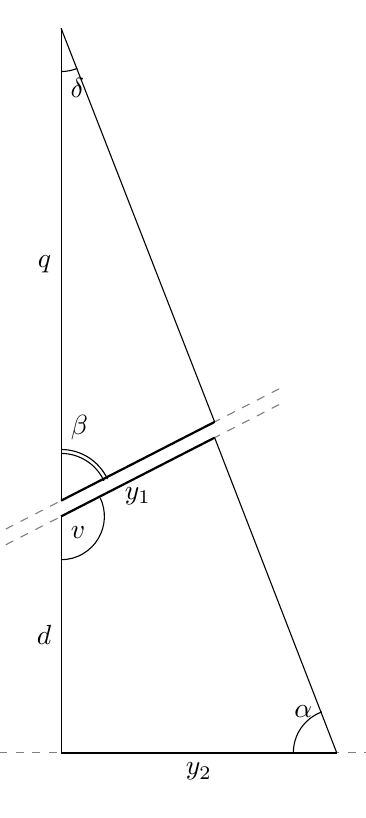
\begin{tikzpicture}[extline/.style={shorten >=-#1,shorten <=-#1},
  extline/.default=1cm,
  axis/.style={extline=1cm, dashed, color=gray}]

\coordinate (origin) at (1,1);
\coordinate (v) at (1,4);
\coordinate (v') at (1,4.2);
\coordinate (p1) at (2.95,5);
\coordinate (p1') at (2.95,5.2);
\coordinate (p2) at (4.5,1);
\coordinate (t) at (1,10.2);

\draw [axis] (origin) -- (p2);
\draw [axis] (v) -- (p1);
\draw [axis] (v') -- (p1');

\draw [thick] (v') -- (p1');

\draw (t) -- (p1') (p1) -- (p2);
\draw (v') -- (t) node [midway, left] {$q$};

\draw (origin) -- (v) node [midway, left] {$d$};
\draw [thick] (v) -- (p1) node [midway, below] {$y_1$};
\draw [thick] (origin) -- (p2) node [midway, below] {$y_2$};

\draw ($(v) + (-90:0.55)$) arc (-90:25:0.55);
\draw ($(v') + (25:0.6)$) arc (25:90:0.6);
\draw ($(v') + (25:0.65)$) arc (25:90:0.65) node [above right] {$\beta$};
\draw ($(t) + (-90:0.55)$) arc (-90:-68:0.55) node [below] {$\delta$};
\draw ($(p2) + (180:0.55)$) arc (180:110:0.55) node [left] {$\alpha$};

\node [below right] at (v) {$v$};
\end{tikzpicture}
\caption{Beregning af $ y_2 $}
\label{localization:trekant}
\end{figure}

Ud fra \cref{localization:trekant} udledes nu $y_2$, så denne er udtrykt ved de tre variable $y_1$, $v$ og $d$.
Først findes de to vinkler $\beta$ og $\delta$:
\begin{align*}
\beta &= 180 - v\\
\delta &= 180-(90 + \beta)\\
&= 180 - (90 + 180 - v)\\
&= v-90
\end{align*}

Herefter benyttes en sinus-relation til bestemmelse af $q$:
$$q = \frac{y_1}{\sin{\delta}}$$

Til sidst kan $y_2$ udledes ved hjælp af tangens:
\begin{align*}
y_2 &= \tan(\delta)(q+d)\\
&= \tan(v-90)\left(\frac{y_1}{\sin(v-90)} + d\right)
\end{align*}

Det skal her bemærkes at den opstillede model udelukkende beskriver koordinater i \'en dimension i planet.
For at kunne finde et punkt i planet er det naturligvis også nødvendigt at håndtere yderligere en koordinat.
Det ønskes hermed at opstille en funktion $f$ der beregner mapping fra $(x_1,y_1)$ til $(x_2,y_2)$, under forudsætning af at $y_1$, $v$ og $d$ kendes på forhånd;
$$f: \mathbb{R} \times \mathbb{R} \times \mathbb{R} \times \mathbb{R} \rightarrow \mathbb{R} \times \mathbb{R}$$
\mikkel[Localization antagelse 2]{Beskriv hvorfor det er ok at antage at førstekoordinaten kan overføres.
Jeg går ud fra at vi laver et eksperiment der viser at det passer - eller at vi finder en anden metode.}
Det antages derfor at $x_1$ = $x_2$, og funktionen $f$ kan nu opstilles:

$$f(x_1,y_1,v,d)=\left(x_1,\;\tan(v-90)\left(\frac{y_1}{\sin(v-90)} + d\right)\right)$$

\part{Design}
\chapter{Robottens design}
% !TeX spellcheck = da_DK
Dette afsnit fokuserer på designet af den robot der har til opgave at navigere rundt i et område for kortlægge det. 

Først vil det blive beskrevet hvordan selve robotten er bygget op med LEGO, og derefter hvordan motorer og sensorer er sat på robotten.

\begin{figure}
\centering
\includegraphics[width=0.6\textwidth]{whalle}
\caption{Endelige design af vores robot.}
\label{robot:opbygning}
\end{figure}




\section{Kroppen}
Kroppen er den centrale komponent, hvor motorene, som styrer henholdsvis hjulene og rotation af sensorerne, er bygget på. 
Samtidig fungere den som det, der "holder robotten sammen".
Desuden er NXT'en også en central del af denne konstruktion.
Placeringen af denne er primært i forhold til funktionelle behov, da der på fronten er knapper til at tænde/slukke og vælge indstillinger med.
Dens placering gør det også nemt at få adgang til dens porte for tilslutning af motor, sensor, opladning samt tilslutning af PC for opdatering af software med mere.

\section{Fremdrift}
Robotten er konstrueret med et \textit{aktivt} hjulsæt, der både giver fremdrift og styring.
Denne funktionalitet opnås ved, at hvert hjul (på hver side af robotten) har sin egen motor, således der kan angives både positiv og negativ fremdrift uafhængigt af hvert hjul.
Dette design gør det muligt at rotere robotten omkring sin egen akse for maksimal mobilitet -- selv på et begrænset område.
Foruden det forreste hjulsæt, er der bagerst på robotten monteret et 'baghjul', hvis eneste funktion er at balancere/stabilisere robotten.
Valget af et hjul til at udføre en sådan funktion er forholdsvis begrænset i \lego, hvorfor valget faldt på et "slæbehjul" med en masse ruller, der gør det muligt for hjulet at rotere i alle retninger.

\section{Sensorer}
Den egentlige funktion af robotten er at tage afstandsmålinger til objekter indenfor sensorernes rækkevidde.
Placeringen af sensorerne er derfor ikke kritisk, da de højst vil give en forskydning af konstant faktor relativ til robottens midte fra deres placering i fronten.
Vigtigere er, at der er 360\degree~udsyn når de roterer, og at robotten ikke er i vejen for målingerne, hvilket er løst ved at montere sensorerne højere end resten af robotten. 

I testen af afstandssensorer (se \cref{sensor:sammenligningIRvsSonar}) viste det sig at de to sensortyper, infrarød og ultrasonisk, havde sammenlignelig præcision, og valget mellem disse to afhænger da af behovet for rækkevidde. 
Den infrarøde sensor kan måle præcist tæt på, mens den ultrasoniske kan måle præcist langt væk.
Til robotten blev det valgt at montere to ultrasoniske sensorer, da det ikke er lige så brugbart at vide tæt robotten er på en mur, som det er at se at der er en mur langt væk når der kortlægges.

\section{Gearing}\label{robot:gearing}
I \cref{sensorer:motorer} fandt vi ud af, at præcisionen på motorerne ikke var høj.
Der var en afvigelse på op til 4\dg, imod den maksimale afvigelse på 1\dg ~nævnt i kravene i \cref{robot:design}.
Dette faktum gav anledning til at udforske mulighederne for at geare motorene for at mindske usikkerheden og øge præcisionen.

\subsection{Simpel Teori}\label{gearing:simpel_teori}
Gearing kan foregå på to måder; geare op eller geare ned.
Det tandhjul, der er knyttet direkte til motoren kalder vi fører-tandhjulet og det tandhjul, der er knyttet til fører-tandhjulet kalder vi for følger-tandhjulet (se evt. \cref{gearing:nedgearing}).

\subsubsection{Nedgearing}
Nedgearing foregår ved at et mindre tandhjul driver et større tandhjul.
Gear rationen (størrelsen af gearing) er styret af antallet af tænder på tandhjulene.
For eksempel vil et 24-tands fører-tandhjul drive et 40-tands følger-tandhjul med ratioen $1:1.667$, hvilket betyder, at der for at give en enkelt følger-omdrejning kræves $1.667$ fører-omdrejninger. 
Det betyder, at motoren der driver fører-tandhjulet skal rotere $\frac{40}{24} = 1 \frac{2}{3}$ omgange for at rotere følger-tandhjulet én omgang og at følger-tandhjulet roterer $\frac{1}{1.667} = 0.6$ omgange pr. omdrejning af fører-tandhjulet.

Til dette projekt bliver der kun gearet ned (jævnfør robottens design på \cref{robot:opbygning}).


\begin{figure}[h]
\centering
\includegraphics[width=.5\textwidth]{gears/op_og_ned}
\caption{Eksempel på (ned-)gearing}
\label{gearing:nedgearing}
\end{figure}

\subsection{Gearing på ultrasonisk sensor}
Dette afsnit fokuserer på den gearing, der er monteret på de ultrasoniske sensorer, som kan ses i \cref{robot:opbygning}.
Denne bruges til at bestemme afstanden til et objekt i en bestemt retning, hvorfor det vil være en fordel at geare motoren ned for at opnå større præcision af denne, når retningen af sensoren skal bestemmes.
Rotationen vil naturligvis foregå langsommere end uden gearing, men da tid ikke er en faktor på nuværende tidspunkt, er det ikke af nogen betydning for at løse problemet.

Gearingen for den ultrasoniske sensor består af i alt 3 forskellige tandhjul (4 i alt), som alle kan ses på \cref{gearing:tandhjul}.

\begin{figure}[h] % De anvendte tandhjul
\centering
\begin{subfigure}[b]{.19\textwidth}
\centering
\includegraphics[width=\textwidth]{gears/worm}
\caption{Snekke}
\label{gearing:snekke}
\end{subfigure}
%\begin{subfigure}[b]{.19\textwidth}
%\centering
%\includegraphics[width=\textwidth]{gears/16-tooth}
%\caption{16-tands}
%\label{gearing:16tand}
%\end{subfigure}
\begin{subfigure}[b]{.19\textwidth}
\centering
\includegraphics[width=\textwidth]{gears/24-tooth}
\caption{24-tands}
\label{gearing:24tand}
\end{subfigure}
\begin{subfigure}[b]{.19\textwidth}
\centering
\includegraphics[width=\textwidth]{gears/40-tooth}
\caption{40-tands}
\label{gearing:40tand}
\end{subfigure}
\caption{De anvendte tandhjul til sensor rotation.}
\label{gearing:tandhjul}
\end{figure}

Den første kombination består af en snekke\cite{snekke} (se \cref{gearing:snekke}) som fører-tandhjul og 24-tands (se \cref{gearing:24tand}) som følger-tandhjul.
Snekken kræver en hel rotation for at flytte én tand på følger-tandhjul, hvilket giver en gear ratio på $1:24$, som betyder, at der kræves 24 hele motor-rotationer for at rotere 24-tands (følger) tandhjulet én omgang.

Den anden kombination består af et 24-tands (se \cref{gearing:24tand}) som fører-tandhjul og et 40-tands (se \cref{gearing:40tand}) som følger-tandhjul, hvilket giver en ratio på $1:1.667$.

Den samlede gear ratio for sensormotoren bliver derfor $1:40$, som beskriver, at der for hver sensor omdrejning kræves 40 motor omdrejninger; hvilket er det samme som:
$$\frac{24}{1} \cdot \frac{40}{24} = 40$$
\chapter{Forsøgsopstilling}
\section{Testmiljø}
I dette afsnit præsenteres det testmiljø, der sat op til at teste robottens færdigheder.

\subsection{Formål}
Formålet med et testmiljø er at bedre kunne kontrollere omgivelserne.
Dette giver mindre unøjagtigheder, ift. hvis det skulle testes i et nyt miljø hver gang, og gør det dermed muligt at sammenligne resultater.

\subsection{Opsætning}\label{testmiljo:opsaetning}
Testmiljøet er opsat vha. papkasser og tape, som man kan se på \cref{testmiljo:perspektiv}.
Størrelsen er $189 \ cm \times 261 \ cm$. 
Denne størrelse er valgt, da dette præcis passer ift. Kinectens billede, som man kan se på \cref{testmiljo:oppefra}.
På \cref{testmiljo:forfra} kan man se hvordan Kinecten er monteret under en loftplade ift. gulvet.

\begin{figure}
\begin{tikzpicture}
\node[anchor=south west,inner sep=0] at (0,0) {\includegraphics[width=\textwidth/2]{./verden/forfra}};
    \draw [->, red, ultra thick] (5.5,10.5) -- (4.2,11.2);
\end{tikzpicture}
\caption{Testmiljøet set forfra. Bemærk Kinecten monteret i en loftsplade (rød pil) med hul til RGB-kameraet.}
\label{testmiljo:forfra}
\end{figure}

\begin{figure}
\includegraphics[width=\textwidth]{./verden/perspektiv}
\caption{Testmiljøet set i perspektiv.}
\label{testmiljo:perspektiv}
\end{figure}

\begin{figure}
\begin{tikzpicture}
\node[anchor=south west,inner sep=0] at (0,0) {\includegraphics{./verden/oppefra}};
    \draw [<->, red, ultra thick] (1.3,0.9) -- (1.5,11.4);
    \node [red, ultra thick] at (2.5,5.5) {189 cm};
    \draw [<->, red, ultra thick] (1.3,0.9) -- (16,1);
    \node [red, ultra thick] at (8, 2) {261 cm};
\end{tikzpicture}
\caption{Testmiljøet set fra Kinecten.}
\label{testmiljo:oppefra}
\end{figure}

\thilemann{Ville det give mening at have et billede af vores occupancy grid?}

\begin{figure}
\includegraphics[width=((\textwidth)/2), clip, trim = 10cm 2cm 10cm 5cm]{./verden/kinect}
\caption{Her kan man se hvordan Kinecten er monteret på loftspladen.}
\label{testmiljo:kinect}
\end{figure}
\part{Implementering}

\part{Konklusion}

\appendix
\part{Appendiks}

\bibliography{bibliography}
\bibliographystyle{plain}
\end{document}